\documentclass[12pt]{article}
\usepackage{lingmacros}
\usepackage{tree-dvips}
\usepackage{graphicx}
\usepackage{grffile}
\usepackage{cite}
\usepackage{float}

\begin{document}
\title{Notes for the navigation project}
\date{2018\\ November}
\author{Raphael Gross}
\maketitle




\section{Introduction}
This is the first project of the Udacity DRL course. My goal for this project is to get a better understanding of Deep Q network (DQN) by implementing some of the latest extensions of DQN~\cite{mnih2015humanlevel} algorithm in pytorch. In order to achieve my goal, I first describe the current state of the art of Deep Q netwok, then I will describe some of the results I obtained on the Banana environment.

Extension of the DQN  algorithm are treated in the following order:

\begin{itemize}
\item DQN~\cite{mnih2015humanlevel}
\item DDQN~\cite{Hasselt2016}
\item Dueling network Architecture~\cite{BellemareDM17}
\end{itemize}


For now, I only covered these 3 items: DQN, DDQN, and dueling. I am currently working on the PER (Prioritized Experience Replay). My plan is to understand, implement and test the next methods too

\begin{itemize}
\item Prioritized experience replay
\item A distributional perspective on reinforcement learning
\item Rainbow: combining improvements in deep reinforcement learning 
\item Distributional reinforcement learning with quantile 
\end{itemize}

\section{Testing environment}
I trained my agent using  variations of the DQN algorithm in order to collect bananas in a large, square world see Figure ~\ref{fig:banana_environment}
A reward of +1 is provided for collecting a yellow banana, and a reward of -1 is provided for collecting a blue banana. Thus, the goal of my agent is to collect as many yellow bananas as possible while avoiding blue bananas.

The state space has 37 dimensions and contains the agent's velocity, along with the ray-based perception of objects around the agent's forward direction. Given this information, the agent has to learn how to best select actions. Four discrete actions are available, corresponding to:

\begin{itemize}
\item move forward.
\item move backward.
\item turn left.
\item turn right.
\end{itemize}
 
The task is episodic. In order to solve the environment, the agent must get an average score of +13 over 100 consecutive episodes.

\begin{figure}[!htbp]
  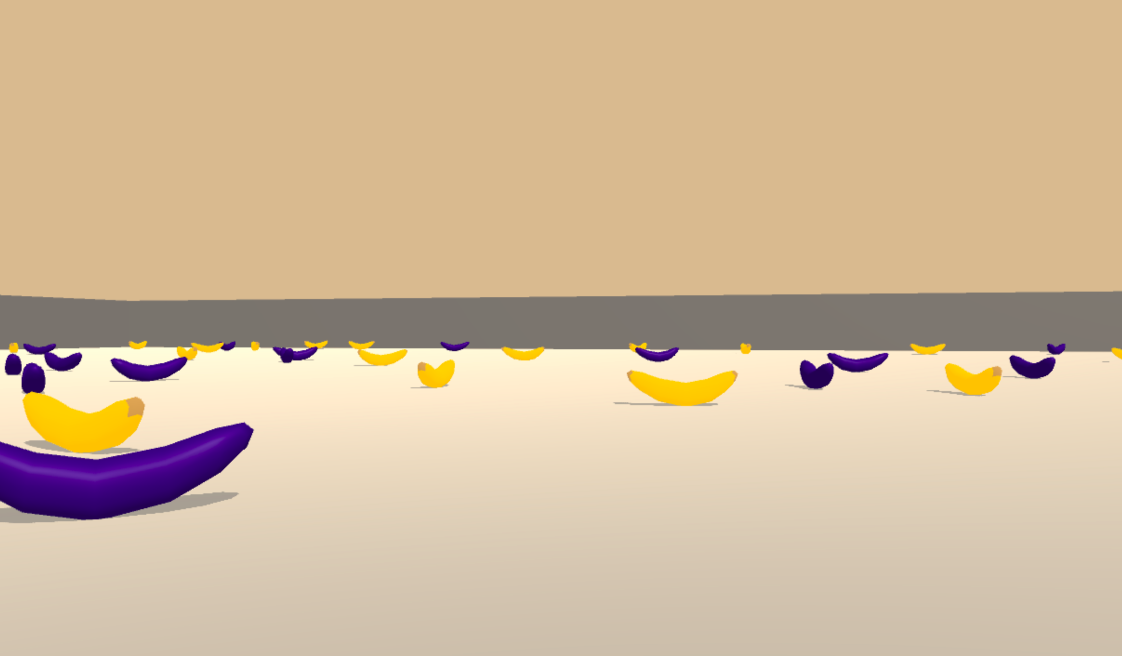
\includegraphics[width=0.9\textwidth]{../PNG/env.png}
  \caption{Banana environment}
  \label{fig:banana_environment}
\end{figure}

\section{State of the Art}
\subsection{Definition}
I consider in this project an agent that interacts with the environment in a sequence of observations $s$, actions $a$, rewards $r$, new states $s'$ such as $(s,a,r,s')$.
At each time step $t$, we have a tuple $(s,a,r,s')$  and each episode is finite. All episodes are terminated in a finite number of time-steps. 
So, we have a well defined Markov decision process. 
 
The agent will interact with the simulator by selecting actions in a way that maximizes future rewards. 
I made the assumption that future rewards are discounted by a factor of $\gamma =0.99$ par time-step. So for a time step $t$ the future reward is:

\begin{equation} 
	R_{t}=\sum_{t'=t}^T \gamma^{t'-t}r_{t'}
\end{equation} 

The optimal action-value function $Q^*(s,a)$ corresponds to the maximum expected return achievable by following any policy after seeing a sequence $s$ and then taking action $a$:

\begin{equation} 
 	Q^*(s,a)=\max_{\pi}\mathrm{E}[R_{t}|s_{t}=s,a_{t}=a,\pi]
\end{equation} 

in which $\pi$ is a policy mapping sequences to actions.

So if the optimal action value $Q^*$ was know for the next observation $s'$ for all possible actions $a'$, the optimal strategy is to select the action $a'$ maximizing the expected value of $r + \gamma Q^*(s',a')$ such as:

\begin{equation} 
 	Q^*(s,a)=\mathrm{E}_{s'}[r + \gamma \max_{a'} Q^*(s',a')|s,a]
\end{equation} 
 
the idea behind this reinforcement problem is to estimate the action-value function by using the Bellman equation as an iterative update:

\begin{equation}
	Q_{i+1}(s,a)=\mathrm{E}_{s^{'}} [r + \gamma \max_{a'} Q^{*}(s',a')|s,a].
\end{equation}

with $Q_{i}$ converging towards $Q^*$ as $i$ goes to infinity. In practice, this is difficult because the action-value function is estimated separately for each sequence, without any generalization. 
This is why a function approximitor $Q(s,a,\theta)$ is used to estimate the action value function $Q^*(s,a)$. 
I used here a $Q$ network for approximator where $\theta$ are the weights of the network.


\subsection*{Deep Q network or DQN}
DQN~\cite{mnih2015humanlevel} combine reinforcement learning with deep neural networks. 
The idea is to used a deep neural network such as a convolutional neural network to approximate the optimal action-value function.
 
However, reinforcement learning is unstable and may even diverge when a nonlinear function approximator such as a neural network is used to represent the action-value function $Q$.
This instability has several causes:

\begin{itemize}
\item correlations present in the sequence of observations.
\item small updates to $Q$ may change the policy and therefore change the data distribution.
\item the correlations between the action-values $Q$ and the target values $r + \gamma \max_{a'} Q(s',a')$.
\end{itemize}

A solution is to use experience replay or memory replay. 
It will randomize the data and remove correlations in the observation sequence. 
It will also smooth the changes in the data distribution. 
During learning, we use mini-batches of experience $(s,a,r,s')$ drawn uniformly at random from a pool of stored samples.

Another possibility that helps in reducing the correlations with the target is to use an iterative update that adjusts the action values towards targets values that are only periodically updated.
The Q function approximator is parametrize such as $Q=Q(s,a,\theta_{i})$ with $\theta_i$ being the weights from the $Q$ neural network at iteration $i$.
At each iteration $i$ we try to reduce the mean-squared error in the Bellman equation, where the optimal target values $r+\gamma  \max_{a'} Q(s',a')$ are substitued with the approximated target values $y=r+\gamma  \max_{a'} Q(s',a',\theta_i^-)$ with $\theta_i^-$ being the weight of the Q network from some previous iteration.
The parameters $\theta^-$ are therefore only updated every $C$ steps and fixed the rest of the time.

The Q learning loss function is defined as:

\begin{equation} 
 	L_{i}(\theta_{i}) =\mathrm{E}_{(s,a,r)}[( E_{s'}[y|s,a]-Q(s,a;\theta_i))^2]
\end{equation}
\begin{equation} 
	L_{i}(\theta_{i}) =\mathrm{E}_{(s,a,r,s')}[(y-Q(s,a;\theta_i))^2]+\mathrm{E}_{(s,a,r)} [\mathrm{V}_{s'}[y]]
\end{equation} 

Since we want to optimize $\theta$ we can ignore the variance of the targets as it is independent of $\theta$.

\begin{equation}  
L_{i}(\theta_{i}) =\mathrm{E}_{(s,a,r,s')}[(r+\gamma  \max_{a'} Q(s',a'; \theta_{i}^- )-Q(s,a;\theta_{i}))^2]
\end{equation} 

The loss function is optimized using a stochastic gradient descent.
The method is also off policy (memory replay). We ensure the exploration of the state and space by using the $\epsilon$-greedy policy.


\subsection*{Double Deep Q network or DDQN}
DQN tend to overestimate the action values especially when the function approximator is inaccurate or the environment is noisy. The problem with the overestimation is that it is not evenly distributed. Therefore, it may result in a modification of the action choice and lead to a sub-optimal policy.

DQN uses the same values both to select and to evaluate an action where DDQN~\cite{Hasselt2016} uses the online weights $\theta_i$ to select an action while the target weights $\theta_i^-$ evaluate the action. 
This idea comes from double Q learning were two value functions are learned.
One set of weights is used to determine the greedy policy action while the other its value.
This change will enable more accurate values to estimate and therefore lead to better policies.

The DQN equation:

\begin{equation}
	y_{DQN}=r+\gamma \max_{a'} Q(s',a',\theta_i^-)
\end{equation}
or 
\begin{equation}
	y_{DQN}=r+\gamma Q(s',argmax_{a'} Q(s',a',\theta_i^-);\theta_i^-)
\end{equation}

The DDQN equation:

\begin{equation}
	y_{DDQN}=r+\gamma Q(s',argmax_{a'} Q(s',a',\theta_i);\theta_i^-)
\end{equation}

\subsection*{Dueling Network architecture}
Compared to regular DQN or DDQN networks, the dueling network architecture~\cite{BellemareDM17} separetes the evaluation of the state value function $V(s)$ and the action advantage function $A(s,a)$ before evaluting via aggregation the state action value function $Q(s,a)$.

So, the dueling network can learn which state is valuable or not without having to learn the effect of each action for each state.
\begin{itemize}
\item $V(s)$: the value of being at that state
\item $A(s,a)$: the advantage of taking that action at that state (how much better is to take this action versus all other possible actions at that state).
\end{itemize}

from the expression of advantage function we have:
\begin{equation}
	Q^{\pi}(s,a)=V^\pi (s) +A^\pi (s,a)
\end{equation}

\begin{equation}
	V^\pi (s)=E_{a \sim \pi(s)}[Q^\pi (s,a)]
\end{equation}

\begin{equation}
	E_{a \sim \pi(s)}[A^\pi (s,a)]=0
\end{equation}

Therefore, for a deterministic policy we have: $Q^*(s,a*)=V(s)$ and $A(s,a*)=0$ for $a^{*}=argmax_a Q(s,a)$.

Compared to DQN and DDQN, the action value function of the dueling network uses a parametrize estimator for $Q(s,a)$:

\begin{equation}
	Q(s,a;\theta,\alpha,\beta)=V(s,\theta,\beta) +A(s,a;\theta,\alpha)
\end{equation}

Even thought, the action value is written under this form, it is not possible to use $V(s,\theta,\beta)$ as a good estimator of $V(s)$ and $A(s,\theta,\alpha)$ as a good estimator of $A(s,a)$. 
The network is build to evaluate $Q(s,a)$ and so it lacks identifiability.

By changing the previous expression a little bit, we can write it such that $V(s,\theta,\beta)=V(s)$ when $a*=argmax_{a'}Q(s,a')$:

\begin{equation}
	Q(s,a;\theta,\alpha,\beta)=V(s,\theta,\beta) +(A(s,a;\theta,\alpha)-max_{a'}A(s,a';\theta,\alpha))
\end{equation}

This formulation does not give any advantage to the chosen action. 
Another possibility which gives more stable results is to subtract by the mean instead of the maximum:
\begin{equation}
	Q(s,a;\theta,\alpha,\beta)=V(s,\theta,\beta) +(A(s,a;\theta,\alpha)-1/{|A|}*\sum_{a'} A(s,a';\theta,\alpha))
\end{equation}

Here, the advantage only needs to change as fast as the mean instead of the optimal action. Also, as we subtract a constant from $A(s,a';\theta,\alpha)$ we do not change the ranking for the action value function estimator $Q(s,a;\theta,\alpha,\beta)$.


\section*{Results} 
\subsection{Models}
The architecute of the network use by the regular DQN and DDQN is composed of 3 linear layers:

\begin{itemize}
\item fc1 : $nn.Linear(state\_size, fc1\_units)$
\item fc2 : $nn.Linear(fc1\_units, fc2\_units)$
\item fc3 : $nn.Linear(fc2\_units, action\_size)$
\end{itemize}
 
where 

\begin{itemize}
\item $state\_size=37$
\item $fc1\_units=64$
\item $fc2\_units=64$
\item $action\_size=4$
\end{itemize}

In the forward pass, $fc1$ and $fc2$ are combined with a $ReLU$ rectifier.
The dueling network version is a bit more complex as we want to express the $Q value$ function as a sum of the advantage function and the state value function $V(s) + (A(s,a) - 1/|A| * sum A(s,a'))$.

\begin{itemize}
\item $fc1 = nn.Linear(state\_size, fc1_units)$
\item $fc2 = nn.Linear(fc1\_units, fc2_units)$
\item $V = nn.Linear(fc2\_units, 1)$
\item $A = nn.Linear(fc2\_units, action_size)$
\end{itemize}


\subsection{Parametric studies for DQN}
In this section, I display some results of the parametric studies I made in order to found the best DQN configuration possible. 

The best result I obtained for DQN was with the next parameters value:
\begin{itemize}
\item MEMORY SIZE = int(1e5) (replay buffer size)
\item BATCH SIZE = 32  (minibatch size)
\item GAMMA = 0.99  (discount factor)
\item TAU = 1e-3  (parameter value used for the soft update of the target weights)
\item LR = 5e-4  (learning rate)
\item UPDATE EVERY = 4  (how often the target network is updated)
\end{itemize}

I will use these values for comparing the results between DQN, DDQN, and the dueling version of DQN and DDQN.

Note: as the first DQN I build manage to solve the system under 500 iteration, I limited the number of episodes to 700 for the parametric studies.  If the agent manages to get a score over 13 for a window of 100 episodes, I considered it as converged (C) otherwise I label it as not converged (N).


\subsubsection{Replay memory size study}
Fixed parameters: batch = 32, tau=1e-3, UPDATE=4, LR=5e-04

\begin{table}[H]
\centering
\begin{tabular}{|c|c|c|c|}
\hline 
{ \textbf{MEM SIZE}} & { \textbf{Max iter}} & { \textbf{score}} & { \textbf{C/N}} \\ \hline
100 & 700 & -     & N \\ \hline
1e3 & 700 & -     & N \\ \hline
1e4 & 423 & 13.01 & C \\ \hline
1e5 & 389 & 13.06 & C \\ \hline
1e6 & 451 & 13.02 & C \\ \hline
\end{tabular}
\caption{Memory size parametric study}
\label{table:Mem}
\end{table}



\subsubsection{Batch size study}
Fixed parameters: MEM = 10000, tau=1e-3, UPDATE=4, LR=5e-04

\begin{table}[H]
\centering
\begin{tabular}{|c|c|c|c|}
\hline
{\textbf{Batch size}} & {\textbf{Max iter}} & {\textbf{score}} & {\textbf{C/N}} \\ \hline
16 & 469 & -      & N \\ \hline
32  & 389 & 13.06 & C \\ \hline
64  & 411 & -     & N \\ \hline
\end{tabular}
\caption{Bath size parametric study}
\label{table:Batch}
\end{table}


\subsubsection{Tau parameter study}
Fixed parameters:MEM = 10000, batch=32, UPDATE=4, LR=5e-04

\begin{table}[H]
\centering
\begin{tabular}{|c|c|c|c|}
\hline
{\textbf{Tau}} & {\textbf{Max iter}} & {\textbf{score}} & {\textbf{C/N}} \\ \hline
1e-2 & 700 & -     & N \\ \hline
1e-3 & 389 & 13.06 & C \\ \hline
1e-4 & 700 & -     & N \\ \hline
\end{tabular}
\caption{Tau parametric study}
\label{table:Tau}
\end{table}


\subsubsection{UPDATE parameter study}
fixed parameters:MEM = 10000, batch=32, Tau=1e-4, LR=5e-04

\begin{table}[H]
\centering
\begin{tabular}{|c|c|c|c|}
\hline
{\textbf{UPDATE}} & {\textbf{Max iter}} & {\textbf{score}} & {\textbf{C/N}} \\ \hline
2  & 428 & 13.08 & N \\ \hline
4  & 389 & 13.06 & C \\ \hline
6  & 447 & 13.00 & N \\ \hline
\end{tabular}
\caption{UPDATE parametric study}
\label{table:UPDATE}
\end{table}


\subsubsection{Learning rate (LR) parameter study}
Study of the LR parameter:
fixed parameters:MEM = 10000, batch=32, Tau=1e-4, UPDATE=4, LR=5e-04

\begin{table}[H]
\centering
\begin{tabular}{|c|c|c|c|}
\hline
{\textbf{LR}} & {\textbf{Max iter}} & {\textbf{score}} & {\textbf{C/N}} \\ \hline
1e-03  & 470 & 13.02 & C \\ \hline
5e-04  & 389 & 13.06 & C \\ \hline
1e-05  & 700 &   -   & N \\ \hline
\end{tabular}
\caption{Learning rate parametric study}
\label{table:LR}
\end{table}


\subsubsection{DQN}
In Figure~\ref{fig:DQN}, I display the score evolution for the DQN method. The DQN method needs at least 436 episodes before converging to a mean score of 13.03.  In Figure~\ref{fig:DQN_smooth}, I plotted a smoothed version of the score evolution.

\begin{figure}[H]
  \centering
  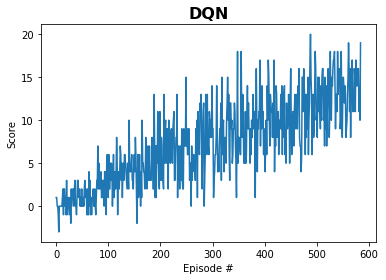
\includegraphics[width=0.5\textwidth]{../PNG/dqn.png}
  \caption{DQN, evolution of the score}
  \label{fig:DQN}
\end{figure}

\begin{figure}[H]
 \centering
  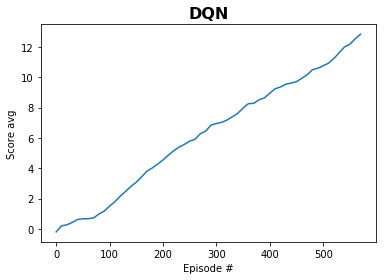
\includegraphics[width=0.5\textwidth]{../PNG/dqn_smooth.png}
  \caption{DQN, evolution of the score averaged over 100 window}
  \label{fig:DQN_smooth}
\end{figure}


\subsubsection{DDQN}
In Figure~\ref{fig:DDQN} and Figure~\ref{fig:DDQN_av}, I show the score evolution for the DDQN method and the smoothed score curve. The DDQN method took 419 episode to reach a score of 13.
\begin{figure}[H]
 \centering
  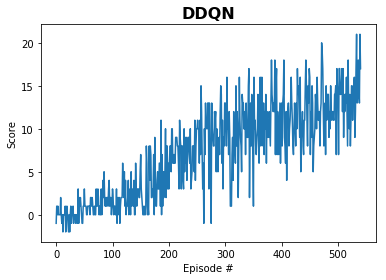
\includegraphics[width=0.5\textwidth]{../PNG/ddqn.png}
  \caption{DDQN, evolution of the score}
  \label{fig:DDQN}
\end{figure}

\begin{figure}[H]
 \centering
  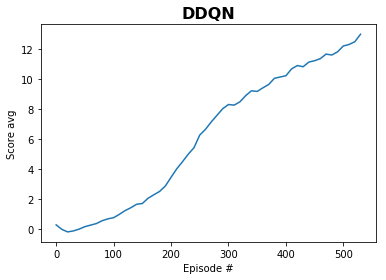
\includegraphics[width=0.5\textwidth]{../PNG/ddqn_smooth.png}
  \caption{DDQN, evolution of the score averaged over 100 window}
  \label{fig:DDQN_av}
\end{figure}


\subsubsection{Dueling DQN}

In Figure~\ref{fig:Duel_DQN}, I plot the score evolution for the DDQN method and in Figure~\ref{fig:Duel_DQN_av} I display the smoothed graph. The dueling version of DQN took 444 episodes before reaching a score of 13 which is a few iterations less than the regular DQN version.

\begin{figure}[H]
 \centering
  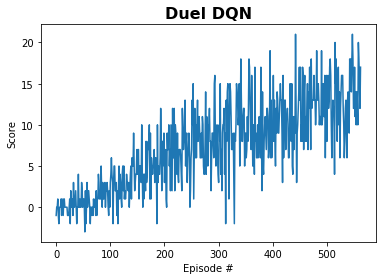
\includegraphics[width=0.5\textwidth]{../PNG/duel_dqn.png}
  \caption{Dueling DQN, evolution of the score}
  \label{fig:Duel_DQN}
\end{figure}

\begin{figure}[H]
 \centering
  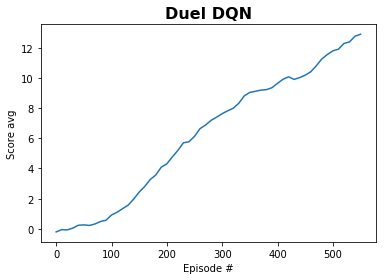
\includegraphics[width=0.5\textwidth]{../PNG/duel_dqn_smooth.png}
  \caption{Dueling DQN, evolution of the average score}
  \label{fig:Duel_DQN_av}
\end{figure}


\subsubsection{Dueling DDQN}
In Figure~\ref{fig:duel_ddqn}, I show the score evolution for the DDQN method and in Figure~\ref{fig:duel_ddqn_av} I plot the smoothed score. The dueling version of DDQN only took 375 episodes which is the best result.

\begin{figure}[H]
 \centering
  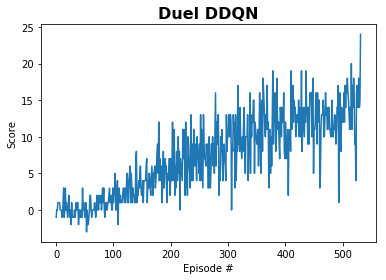
\includegraphics[width=0.5\textwidth]{../PNG/duel_ddqn.png}
  \caption{Dueling DDQN, evolution of the score}
  \label{fig:duel_ddqn}
\end{figure}

\begin{figure}[H]
 \centering
  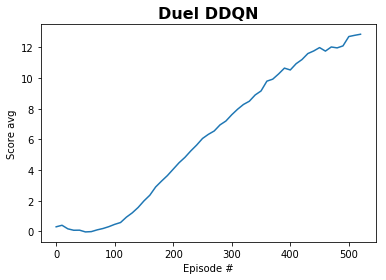
\includegraphics[width=0.5\textwidth]{../PNG/duel_ddqn_smooth.png}
  \caption{Dueling DDQN, evolution of the average score}
  \label{fig:duel_ddqn_av}
\end{figure}


\subsubsection{Comparison}
In Figure~\ref{fig:comparison}, I plot the smoothed score evolution for each method. 
We can see that the dueling version of DQN and DDQN are slower to learn at the beginning but tend to learn at a faster speed later on. 
Finally, we got the more improvement by switching from DQN to DDQN.

\begin{figure}[H]
 \centering
  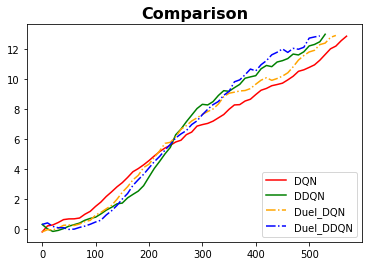
\includegraphics[width=0.5\textwidth]{../PNG/Comparison.png}
  \caption{Comparison of the average score for DQN, DDQN, dueling DQN and dueling DDQN}
  \label{fig:comparison}
\end{figure}

\section{Future developments and improvements}
As I mentioned in the introduction I covered DQN, DDQN, and dueling network. I am currently working on the PER (Prioritized Experience Replay) and my plan is to implement and test the next methods too:

\begin{itemize}
\item Prioritized experience replay
\item A distributional perspective on reinforcement learning
\item Rainbow: combining improvements in deep reinforcement learning 
\item Distributional reinforcement learning with quantile 
\end{itemize}

There are other several things that I did not check for now and that could also improve my results. One of them would be to change the size of the network such as the number of hidden layers.

\bibliography{bib}{}
\bibliographystyle{plain}

\end{document}


